\documentclass[twoside]{article}
\setlength{\oddsidemargin}{0.25 in}
\setlength{\evensidemargin}{-0.25 in}
\setlength{\topmargin}{-0.6 in}
\setlength{\textwidth}{6.5 in}
\setlength{\textheight}{8.5 in}
\setlength{\headsep}{0.75 in}
\setlength{\parindent}{0 in}
\setlength{\parskip}{0.1 in}
\newcommand{\eqdef}{:\mathrel{\mathop=}}
\newcommand{\norm}[1]{\left\lVert #1 \right\rVert}

%
% ADD PACKAGES here:
%
\usepackage{algorithm}
\usepackage[noend]{algpseudocode}
\usepackage{amsmath,amsfonts,graphicx}

%
% The following commands set up the lecnum (lecture number)
% counter and make various numbering schemes work relative
% to the lecture number.
%
\newcounter{lecnum}
\renewcommand{\thepage}{\thelecnum-\arabic{page}}
\renewcommand{\thesection}{\thelecnum.\arabic{section}}
\renewcommand{\theequation}{\thelecnum.\arabic{equation}}
\renewcommand{\thefigure}{\thelecnum.\arabic{figure}}
\renewcommand{\thetable}{\thelecnum.\arabic{table}}

%
% The following macro is used to generate the header.
%
\newcommand{\lecture}[4]{
   \pagestyle{myheadings}
   \thispagestyle{plain}
   \newpage
   \setcounter{lecnum}{#1}
   \setcounter{page}{1}
   \noindent
   \begin{center}
   \framebox{
      \vbox{\vspace{2mm}
    \hbox to 6.28in { {\bf Advanced Machine Learning
	\hfill Fall 2020} }
       \vspace{4mm}
       \hbox to 6.28in { {\Large \hfill Lecture #1: #2  \hfill} }
       \vspace{2mm}
       \hbox to 6.28in { {\it  #3 \hfill  #4} }
      \vspace{2mm}}
   }
   \end{center}
   \markboth{Lecture #1: #2}{Lecture #1: #2}

   {\bf Note}: {\it LaTeX template courtesy of UC Berkeley EECS dept.}

   {\bf Disclaimer}: {\it These notes are adapted from ETH's Advanced Machine Learning Course,  Bishop's "Pattern Recognition and Machine Learning" book and Joachims et al.'s paper: "Predicting Structured Objects with Support Vector Machines"}
   \vspace*{4mm}
}
%
% Convention for citations is authors' initials followed by the year.
% For example, to cite a paper by Leighton and Maggs you would type
% \cite{LM89}, and to cite a paper by Strassen you would type \cite{S69}.
% (To avoid bibliography problems, for now we redefine the \cite command.)
% Also commands that create a suitable format for the reference list.
\renewcommand{\cite}[1]{[#1]}
\def\beginrefs{\begin{list}%
        {[\arabic{equation}]}{\usecounter{equation}
         \setlength{\leftmargin}{2.0truecm}\setlength{\labelsep}{0.4truecm}%
         \setlength{\labelwidth}{1.6truecm}}}
\def\endrefs{\end{list}}
\def\bibentry#1{\item[\hbox{[#1]}]}

%Use this command for a figure; it puts a figure in wherever you want it.
%usage: \fig{NUMBER}{SPACE-IN-INCHES}{CAPTION}
\newcommand{\fig}[3]{
			\vspace{#2}
			\begin{center}
			Figure \thelecnum.#1:~#3
			\end{center}
	}
% Use these for theorems, lemmas, proofs, etc.
\newtheorem{theorem}{Theorem}[lecnum]
\newtheorem{lemma}[theorem]{Lemma}
\newtheorem{proposition}[theorem]{Proposition}
\newtheorem{claim}[theorem]{Claim}
\newtheorem{corollary}[theorem]{Corollary}
\newtheorem{definition}[theorem]{Definition}
\newenvironment{proof}{{\bf Proof:}}{\hfill\rule{2mm}{2mm}}

% **** IF YOU WANT TO DEFINE ADDITIONAL MACROS FOR YOURSELF, PUT THEM HERE:

\newcommand\E{\mathbb{E}}

\begin{document}
%FILL IN THE RIGHT INFO.
%\lecture{**LECTURE-NUMBER**}{**DATE**}{**LECTURER**}{**SCRIBE**}
\lecture{8}{Soft Margin and Structured SVMs }{}{}
%\footnotetext{These notes are partially based on those of Nigel Mansell.}

% **** YOUR NOTES GO HERE:

% Some general latex examples and examples making use of the
% macros follow.  
%**** IN GENERAL, BE BRIEF. LONG SCRIBE NOTES, NO MATTER HOW WELL WRITTEN,
%**** ARE NEVER READ BY ANYBODY.


\section{Soft Margin SVM} 
So far, we have assumed that the training data points are linearly separable in the feature space. In practice, however, the class conditional distributions may overlap, in which case exact separation of the training data can lead to poor generalization. We therefore need a way to modify support vector machines so as to allow some of the training points to be misclassified. \\

To do this, we introduce slack variables $\xi_{i} \geq 0$ where $i=1,\ldots,N$. These are defined by $\xi_{i} = 0$ for data points that are on or inside the correct margin boundary and $\xi_{i}= \lvert t_{i} - y(x_{i}) \rvert$ for other points. Thus a data point $x_{i}$ that is on the decision boundary $y(x_{i})=0$ will have $\xi_{i} = 1$, and points with $\xi_{i} > 1$ will be misclassified. \\

\begin{figure}[h]
\caption{Illustration of the slack variables.}
\centering
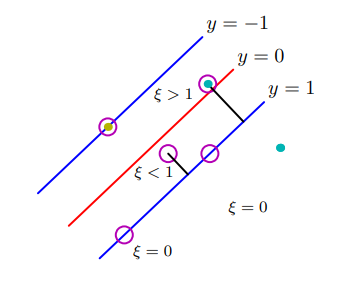
\includegraphics[width=0.39\textwidth]{img/slack.png}
\end{figure}

The exact classification constraints are then replaced with:

\begin{align*}
       t_{i} y(x_{i}) \geq 1 - \xi_{i} \ \ i=1,\ldots,N \\        
        \xi_{i} \geq 0 \ \ i=1,\ldots,N\\ 
\end{align*}

Our goal is now to maximize the margin while softly penalizing points that lie on the wrong side of the margin boundary. We therefore minimize:

\begin{equation*}
\begin{aligned}
& \underset{w,b,\xi}{\text{min}}
& & \dfrac{1}{2} \norm{w}^2 + C \sum_{i=1}^{N} \xi_{i}\\
& \text{subject to}
& & 1 - \xi_{i} - t_{i} (w^T \phi(x_{i}) +b)  \leq 0, \; i = 1, \ldots, N \\
&&& - \xi_{i} \leq 0, \; i = 1, \ldots, N
\end{aligned}
\end{equation*}

The parameter $C > 0$ controls the trade-off between the slack variable penalty and the margin (training error vs model complexity). In the limit $C \xrightarrow{} \infty $ we will recover the "hard" margin SVM. 

\subsection{Dual Problem}
It is trivial to show that Slater's condition holds since the constraints are affine functions. Therefore, strong duality holds and we can move to the Lagrangian:

\begin{equation*}
    \mathcal{L}(w,b,\xi,a,u) = 
    \dfrac{1}{2} \norm{w}^2 + C \sum_{i=1}^{N} \xi_{i} + \sum_{i=1}^{N} a_{i} \{ 1 - \xi_{i} - t_{i} (w^T \phi(x_{i}) +b) \}
    - \sum_{i=1}^{N} u_{i}\xi_{i}
    \end{equation*}

Furthermore, the corresponding KKT conditions are:
\begin{align}
        a_{n} \geq 0 \\       
        t_{n}y(x_{n}) -1 +\xi_{n} \geq 0 \\
        a_{n}(t_{n}y(x_{n}) -1 +\xi_{n} ) = 0
        \\
        u_{n} \geq 0 \\
        \xi_{n} \geq 0 \\
        u_{n}\xi_{n} = 0
\end{align}


We now optimize out $w,b,\xi_{i}$:

\begin{align*}
        \frac{\partial{\mathcal{L}}}{\partial{w}} = 0 \implies w = \sum_{i=1}^{N} a_{i}t_{i}\phi(x_{i}) \\       \frac{\partial{\mathcal{L}}}{\partial{b}} = 0 \implies \sum_{i=1}^{N} a_{i}t_{i} = 0 \\
        \frac{\partial{\mathcal{L}}}{\partial{\xi_{i}}} = 0 \implies 
        a_{i} = C - u_{i}
\end{align*}

Using the previous results from "hard" margin SVM together with the above  results, we can  eliminate $w,b,\xi_{i}$ from the Lagrangian. We obtain the dual Lagrangian function which is identical to the "hard" margin one, except that the constraints are somewhat different:


\begin{align*}
         \mathcal{L}(\xi,a,u) = \sum_{i=1}^{N} a_{i}  - \dfrac{1}{2}
    \sum_{i=1}^{N} { \sum_{j=1}^{N} a_{i} a_{j} t_{i} t_{j} \phi(x_{i})^T \phi(x_{j})} + C \sum_{i=1}^{N} \xi_{i} - \sum_{i=1}^{N} a_{i} \xi_{i} -
         \sum_{i=1}^{N} u_{i} \xi_{i} \\       
          \mathcal{L}(\xi,a,u) = \sum_{i=1}^{N} a_{i}  - \dfrac{1}{2}
    \sum_{i=1}^{N} { \sum_{j=1}^{N} a_{i} a_{j} t_{i} t_{j} \phi(x_{i})^T \phi(x_{j})} +  \overbrace{\sum_{i=1}^{N} \xi_{i} (a_{i} + u_{i}) - \sum_{i=1}^{N} a_{i} \xi_{i} -
         \sum_{i=1}^{N} u_{i} \xi_{i}}^\text{=0} 
        \end{align*}

This gives the dual representation of the soft margin SVM problem:
\begin{equation*}
\begin{aligned}
& \underset{a}{\text{max}}
& & \sum_{i=1}^{N} a_{i}  - \dfrac{1}{2}
    \sum_{i=1}^{N} { \sum_{j=1}^{N} a_{i} a_{j} t_{i} t_{j} \phi(x_{i})^T \phi(x_{j})}\\
& \text{subject to}
& & 0 \leq a_{i} \leq C  , \; i = 1, \ldots, N \\
&&& \sum_{i=1}^{N} a_{i}t_{i} = 0
\end{aligned}
\end{equation*}

Where the first constraint comes from the fact that $a_{i} = C - u_{i}$ and $a_{i} \geq 0, u_{i} \geq 0$ must be satisfied (KKT).
\\

We can now interpret the resulting solution:
\begin{itemize}
    \item data points for which $a_{i} = 0$: they do not contribute to the predictive model.
    \item data points for which $0 < a_{i} < C$: lie on the margin since $a_{i} < C \implies u_{i} > 0 \implies \xi_{i} = 0$  \\ where the last implication comes from complementary slackness (8.6)
    \item data points for which $a_{i} = C$: lie inside the margin and can either be correctly classified if $\xi_{i} \leq 1$ or misclassifed if $\xi_{i} > 1$
\end{itemize}
\newpage


\section{Structured SVMs}
Consider the problem of natural language parsing illustrated in Figure 8.2. A parser takes as input a natural
language sentence, and the desired output is the parse tree
decomposing the sentence into its constituents. How can we take, say,
an SVM and learn a rule for predicting trees?

\begin{figure}[h]
\caption{Predicting trees in natural language parsing.}
\centering
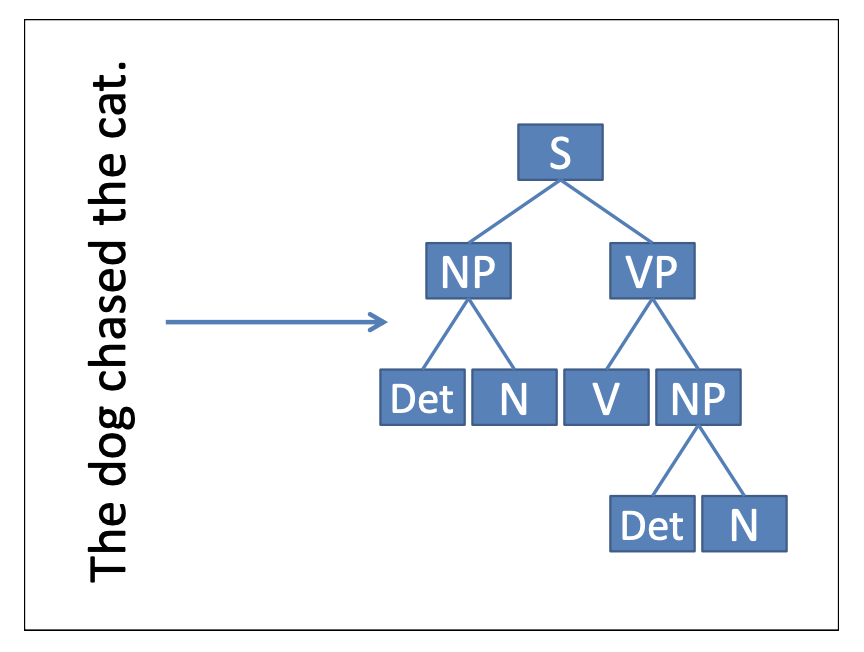
\includegraphics[width=0.39\textwidth]{img/syn_tree.png}
\end{figure}


Obviously, this question arises not only for learning to
predict trees, but similarly for a variety of other structured
and complex outputs. Structured output prediction is the
name for such learning tasks, where one aims at learning
a function $h : X \rightarrow Y$ mapping inputs $x \in X$ to complex
and structured outputs $y \in Y$. 
\\ \\ On an abstract level, a structured prediction task is much like
a multi-class learning task. Each possible structure $y \in Y$
(e.g. parse tree) corresponds to one class (see Figure 8.3), and
classifying a new example $x$ amounts to predicting its correct
“class”. 

\begin{figure}[h]
\caption{Structured output prediction as a multiclass problem.}
\centering
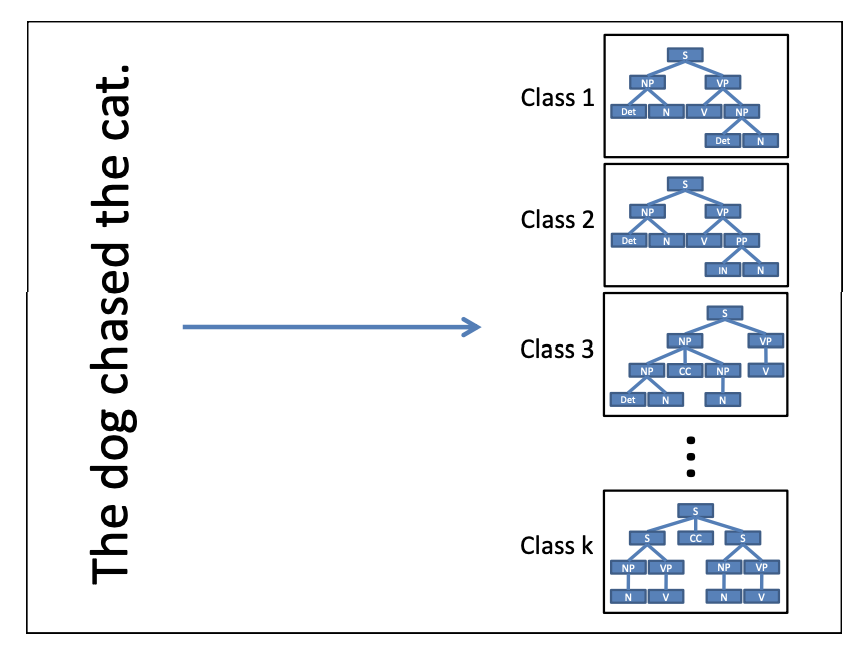
\includegraphics[width=0.39\textwidth]{img/syn_out.png}
\end{figure}

While the following derivation of structural SVMs
starts from multi-class SVMs, there are three key problems
that need to be overcome. \textbf{All of these problems arise from
the huge number $\mathbf{|Y|}$ of classes}. 
\newpage

\subsection{Problem 1: Structural SVM Formulation}
We start the derivation of the structural SVM from the multi-class SVM. These multi-class SVMs use one weight vector $\mathbf{w_{y}}$ for each class $\mathbf{y}$. Each input
$\mathbf{x}$ now has a score for each class $\mathbf{y}$ via $\mathbf{f(x,y) = w_{y} \phi(x)}$.
Here $\mathbf{\phi(x)}$ is a vector of binary or numeric features extracted
from $\mathbf{x}$. Thus, every feature will have an additively weighted
influence in the modeled compatibility between inputs $\mathbf{x}$ and
classes $\mathbf{y}$. To classify $\mathbf{x}$, the prediction rule $\mathbf{h(x)}$ then simply
chooses the highest-scoring class:

\begin{equation}
    h(x) = \max_{y \in Y} f(x,y)
\end{equation}

as the predicted output. This will result in the correct prediction $\mathbf{y}$ for input $\mathbf{x}$ provided the weights $\mathbf{w = (w_{1}, . . . , w_{k})}$
have been chosen such that the inequalities $\mathbf{f(x,y_{i}) < f(x, y)}$
hold for all incorrect outputs $\mathbf{y_{i} \not =  y}$. \\

The first challenge in using (2) for structured outputs is that, while there is generalization across inputs $\mathbf{x}$, there is no generalization across outputs. This is due to having a
separate weight vector $\mathbf{w_y}$ for each class $\mathbf{y}$. Furthermore,
since the number of possible outputs can become very large (or infinite), naively reducing structured output prediction
to multi-class classification leads to an undesirable blow-up
in the overall number of parameters and in the overall number of inequalities, which is $\mathbf{n(k-1)}$. \\

The key idea in overcoming these problems is to extract
features from input-output pairs using a so-called joint feature map $\mathbf{\Psi(x, y)}$ instead of $\mathbf{\Psi(x)}$. These joint features will allow us to generalize across outputs and to define meaningful scores even
for outputs that were never actually observed in the training data. At the same time, since we will define compatibility
functions via $\mathbf{f(x, y) = w\cdot \Psi(x, y)}$, the number of parameters will simply equal the number of features extracted via
$\mathbf{\Psi}$, which may not depend on $\mathbf{|Y|}$. One can then use the formulation in (2) with the more flexible definition of $\mathbf{f}$ via $\mathbf{\Psi}$ to
arrive at the following (hard-margin) optimization problem:

\begin{equation*}
\begin{aligned}
& \underset{\textbf{w}}{\text{min}}
& & \dfrac{1}{2} \norm{w}^2  \\
& \text{subject to}
& & w \cdot \Psi(x_{i},y_{i}) - w \cdot \Psi(x_{i},y) \geq 1 , \;\forall i, y \not = y_{i}
\end{aligned}
\end{equation*}

In other words, find a weight vector $\mathbf{w}$ of an input-output compatibility function $\mathbf{f}$ that is linear in some joint feature map $\mathbf{\Psi}$
so that on each training example it scores the correct output
higher by a fixed margin than every alternative output, while
having low complexity (i.e. small norm $\norm{w}$). Note that the
number of linear constraints is still $n(|Y| -1)$. The design of the features $\mathbf{\Psi}$ is problem-specific, and it is a
strength of the developed methods to allow for a great deal of flexibility in how to choose it.

\subsection{Problem 2: Inconsistent Training Data}
So far we have tacitly assumed that the optimization problem has a solution, i.e. there exists a weight vector
that simultaneously fulfills all margin constraints. In practice this may not be the case, either because the training
data is inconsistent or because our model class is not powerful enough. If we allow for mistakes, though, we must
be able to quantify the degree of mismatch between a prediction and the correct output, since usually different incorrect predictions vary in quality. This is exactly the role
played by a loss function, formally $ \Delta : Y \times Y \rightarrow \mathbb{R}$, where
$\mathbf{\Delta(y_{i},y)}$ is the loss (or cost) for predicting $\mathbf{y}$, when the correct output is $\mathbf{y_{i}}$. Like the choice of $\mathbf{\Psi}$, defining $\mathbf{\Delta}$
is problem-specific. One can convert this back into a
quadratic program as follows:

\begin{equation*}
\begin{aligned}
& \underset{\textbf{w}, \xi_{i} \geq 0}{\text{min}}
& & \dfrac{1}{2} \norm{w}^2 + \dfrac{C}{n} \sum_{i=1}^{n} \xi_{i} \\
& \text{subject to}
& & w \cdot \Psi(x_{i},y_{i}) - w \cdot \Psi(x_{i},y) \geq  \Delta(y_{i},y) - \xi_{i} , \;\forall i, y \not = y_{i}
\end{aligned}
\end{equation*}

Note that we added the $\mathbf{\dfrac{1}{n}}$ term, this is a guarantee that we are minimizing the empirical risk:

\begin{theorem}
If $w^*,\xi^*$ are optimal, then the empirical risk of $w^*$ with respect to $\mathbf{\Delta}$:
\begin{equation*}
    \dfrac{1}{n} \sum_{i=1}^{n}\Delta(y_{i},h_{w^*}(x_{i})) \leq \dfrac{1}{n} \sum_{i=1}^{n} \xi_{i}^*
\end{equation*}
\end{theorem}
\begin{proof}
Suffices to prove that  $\Delta(y_{i},h_{w^*}(x_{i})) \leq \xi_{i}^*,  \; \forall i$ \\

If $h_{w^*}(x_{i}) = y_{i}$, then $\Delta(y_{i},h_{w^*}(x_{i})) = 0 \leq \xi_{i}^*$ \\

If $h_{w^*}(x_{i}) = y \not = y_{i}$, then:
\begin{align*}
       w^{*T}\cdot \Psi(x_{i},y_{i}) < w^{*T} \cdot \Psi(x_{i},y) \implies w^{*T}\cdot \Psi(x_{i},y_{i}) - w^{*T} \cdot \Psi(x_{i},y) = \delta < 0\\      \delta + \xi_{i}^* \geq \Delta(y_{i},y)  \implies  \xi_{i}^* \geq \Delta(y_{i},y)  , \;\forall i \; \text{(from the optimization constraint)}
\end{align*}
\end{proof}


\subsection{Problem 3: Efficient Training}

Last, but not least, we need a training algorithm that finds
the optimal $\mathbf{w}$ solving the quadratic program. Since
there is a constraint for every incorrect label $\mathbf{y}$, we cannot
enumerate all constraints and simply give the optimization problem to a standard QP solver. Instead, we propose to use the cutting-plane Algorithm 1. The key idea is to iteratively construct
a working set of constraints $\mathbf{W}$ that is equivalent to the full
set of constraints  up to a specified precision $\mathbf{\epsilon}$.

\begin{figure}[h]
\centering
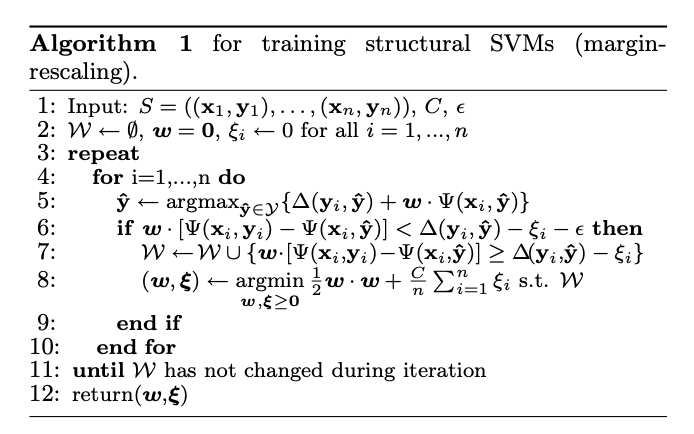
\includegraphics[width=0.52\textwidth]{img/struct_algo.png}
\end{figure}


Starting
with an empty $\mathbf{W}$ and $\mathbf{w=0}$, Algorithm 1 iterates through
the training examples. For each example, the $\mathbf{argmax}$ in Line 5 finds the most violated constraint of the quadratic
program. If this constraint is violated by more than $\mathbf{\epsilon}$ (Line 6), it is added to the working set $\mathbf{W}$ in Line 7 and a
new $\mathbf{w}$ is computed by solving the quadratic program over
the new $\mathbf{W}$ (Line 8). The algorithm stops and returns the
current $\mathbf{w}$ if $\mathbf{W}$ did not change between iterations.\\ 

\textbf{But how long does
it take to terminate?} It can be shown that Algorithm 1
always terminates in a polynomial number of iterations that is independent of the cardinality of the output space $|Y|$. In
fact, a refined version of Algorithm 1  always terminates after adding at most $O(C\epsilon^{-1})$ constraints to $W$. Note that the number of constraints
is not only independent of $|Y|$, but also independent of the
number of training examples $n$, which makes it an attractive
training algorithm even for conventional SVMs. \\
While the number of iterations is small, the $\mathbf{argmax}$ in
Line 5 might be expensive to compute. In general, this is
true, but note that this $\mathbf{argmax}$ is closely related to the
$\mathbf{argmax}$ for computing a prediction $\mathbf{h(x)}$. It is therefore
called the “loss-augmented”inference problem, and often the
prediction algorithm can be adapted to efficiently solve the
loss-augmented inference problem as well.

\end{document}



